\documentclass{article}
    \title{Garden of Eden}
    \author{William B. Jackson}
    \date{May 30, 2014}

    \newcommand{\tab}{\hspace*{2em}}
    \usepackage{fullpage}
    \usepackage{alltt}
    \usepackage{natbib}
    \usepackage{graphicx}
    \usepackage{amsmath}

    % `` instead of left quote "

\begin{document}
    \maketitle

    \setcounter{tocdepth}{2}
    \tableofcontents

    % Acknowledgements: Balkcom, friends, mom, uncle john


    \section{Abstract} % NOTE: this is really bad and needs to be re-written.
    \tab Garden of Eden is an exercise in procedural generation of lifelike worlds. It randomly
generates a forest scene of realistically shaped and proportioned asymmetric trees on top of a
simple topographical map. This map is then rendered in an HTML5 3D canvas, with support for user
navigation. The end result of this project is a sort of game, though without any goal, narrative, or creative purpose.
It is simply a static rendering of a natural environment, open for exploration, closed to
manipulation, exploring how users find visual pleasure and meaning in virtual environments. The
passive interaction of the user is integral to this simulation, as it reflects how one would observe a
natural environment; by forcing the user into the same perspective from which they view actual
forest environments, Garden of Eden explores the concept of “natural”, the distinction between
real and virtual, and the user's sense of place. All software packages are offered open source,
with detailed documentation, for users wishing to create their own arboreal experience.
 
    % Intro: what is the need? motivation, difficulty, etc.
    % Abs: ad for the paper, shorter,  mirrors introduction, fewer results and motivation
    % Refocus on engineering

    \section{Introduction}
    \tab This paper outlines in detail a set of software packages that, when used together, render
a 3D visualisation of a forest scene. The packages are provided separately as well, allowing users
to take advantage of them in order to render their own terrain, trees, and forests. The terrain
construction uses a simple midpoint displacement algorithm\cite{fournier82} to create fractal
surfaces with the feel of a natural topography. The tree generator uses Lindenmeyer
systems\cite{abp96}, called henceforth L-Systems, to define recursive replacment rules for
branching. They then use a LOGO-style turtle graphics wrapper for the Three.js library to render
the tree on an HTML5 canvas, allowing for local hardware acceleration via WebGL.

    \tab The paper is broken up into several parts, first discussing the terrain and trees, then
the state of the project. The terrain section is more sparse, reflecting my focus on the more
verbose tree section; both, however, begin by describing the algorithms implemented and rationale
for their use. The state of the project is discussed by mentioning a few current issues, then going
in to depth on some future improvements to the project as a whole.

    \tab Trees are fascinating in their delicate complexity: a barren tree on a cold winter
day criss-crosses in a spider's web of twigs, simultaneously drawing the eye and losing it in the
intricate patterns of its branches. This visual pleasure is my inspiration for the project: my
intention is to use computers and botanically-influenced algorithms as an engine of fascinating
complexity. The software is open source, allowing users to use it freely for their own purposes. It
could be used to compute the geometry for any visual need: a user might use these trees to fill out
a CGI scene, adding interesting trees to an otherwise sparse landscape. The user is bound only by
the terms of the GPL v3.0 in how they use this software.

    \tab I would like to thank Professor Devin Balkcom, my advisor, for enabling me to work on this
project, even though it is outside of your field of interest. I would like to thank my parents, as
well, for giving me a childhood spent climing trees and a college where I could build them.
\emph{If you do not look, you will not see.}

    \section{Related Work}
        % Phrase any assertions with relation to thesis as things done
        % Phrase tentatively if I didn't do it
    \tab A significant body of work relating to natural feature generation exists in the video game
industry. Minecraft\cite{minecraft}, for example, uses advanced terrain and feature generation
techniques to programmatically create such natural features as mountain ranges, cave systems, chasms,
coasts, and flora biomes, as well as artifical features such as temples, villages, and mine shafts.
It achieves visually impressive scenes using simplified graphics, resulting in a stylised look rather
than striving for verisimillitude. Another game worth mentioning in this context is
Proteus\cite{proteus}, a small-scale ``game of audio-visual exploration and discovery" that allows
users to explore a highly-stylized generated island. There are many other games that use feature
generation techniques, either as the creative force of the game world or to fill in between created
features; I mention these two primarily because, through both gameplay and simple, yet striking,
natural scenery, they served as inspiration for this project.

    \tab B. Mandelbrot and J. Van Ness\cite{mandelbrot68} propose using \emph{fractal Brownian Motion}, a
function that uses the idea of brownian motion with a degree of randomness
to produce a natural-looking surface. The FBM algorithm, however, is very mathematically complex, and
as far simpler algorithms exists that offer adequate approximations to its output, it will not be
implemented. As both FBM and the algorithm implemented use the same constants to describe the
generated surface, however, an understanding of the workings of FBM is valuable to proper
construction of fractal terrains.

    \tab H. Hnaidi et al.\cite{hnaidi10} uses manual seeding of feature curves combined with
a model of material diffusion to generate feature-based, eroded terrain in a single step. The algorithm
propsed requires more manual input than the midpoint displacement algorithm, and is thus less
desirable for the purposes of Garden of Eden. A similar algorithm could be implemented, however,
that randomly places feature curves to achieve a more striking, feature-based landscape.

    \tab J. Bloomenthal\cite{bloomenthal85} discusses detailed visual aspects of tree
generation, specifically the maple tree, assuming a realistic skeleton is available. Thus, he
mostly describes some of the finer visual details in modeling trees, such as branch continuity and
bark texture modeling. Some of his methods have been considered as extensions, but generally, as
his work was focused on the details of computer visualisations of trees, it is out of scope.

    \tab J. Arvo et al. suggest a method for plant rendering that uses cellular automata and ray tracing
to guide the growth of plant skeletons\cite{arvo88}. They discusse how the propsed method
might be applied to grow ivy and grass, but also describe it as it might be used to generally grow
plants, citing specifically tree generation as the prior work from which it builds. The proposed
method is heavily focused on the plant's interaction with the environment, and has tropism,
a subject discussed in the extensions to this project, built in to the generation. Future work
might examine how such methods could be used, either in conjunction with or instead of the
recursive strategy employed.

   \tab P. de Reffye et al. discusses a model for plant generation that draws on the actual botanical 
methods for plant growth\cite{dereffye88}. The methods use stochastic states for growth and time
steps to simulate the actual growth progression, drawing from data in a library of plant
information to construct a wide variety of different trees. The method described might be well
integrated with the above cellular automata geometry construction, and suggests ways by which
different species could be emulated.

    \tab Jason Weber\cite{weber95} draws from an array of previous work to develop a model for the
visual depiction of trees, using extensive data to render a wide variety of flora. His paper
displayed the variability of the model with pictures of trees of several species. This accuracy was
a combination of modeling a
large number of growth affectors as well as extensive research and observation of trees to obtain
a reliable set of constants, many of which could be used to improve the current ranges used for
parameter variation, discussed later.

    \section{Terrain}
        \subsection{Midpoint Displacement}
    \tab The classic method of generating terrain maps is by using a fractal Brownian Motion
function\cite{mandelbrot68}. The function is fairly complex in theory; it can be approximated,
however, with an algorithm called the \emph{midpoint displacement algorithm}\cite{fournier82}. The
midpoint displacement algorithm, also known as the diamond-square algorithm, is an easy way to
generate surface height maps for terrain. The algorithm is as follows\cite{martz97}:
    \begin{verbatim}
Loop while quadrilateral side is at least 1
    // Square step
    For each discrete square of given quadrilateral side length
        Get midpoint of square
        Calculate random offset as a random number in a specified range times a scale
        Midpoint becomes average of square's corners plus random offset

    // Diamond step
    For each discrete diamond defined by the square step's calculated midpoints
        Get midpoint of diamond
        Calculate random offset as a random number in a specified range times a scale
        Midpoint becomes average of diamond's corners plus random offset

    Decrease scale by a constant fraction
    Half quadrilateral side

    \end{verbatim}

    \tab The algorithm is works well to generate fractal surfaces, and allows for a decent amount
of control over the percieved ``roughness" of the resultant surface in how one defines $H$, the fractal
dimension. However, there are well-documented artifacts, notably for steeper surfaces.
These factors can be mitigated somewhat with careful selection of constants, discussed below.


        \subsection{Gaussian Filter}
    \tab The generated terrain from the above algorithm, while showing appropriate large sloping,
is far too bumpy on the player scale to be appropriate for a navigated terrain map. The small
bumps result in constant jostling of the player camera, which is maintained at a constant distance
\verb|CAMERA_HEIGHT| above the terrain. To address this problem, the terrain height map is passed
through a low-pass filter, which maintains the low frequency noise--the larger hills and
valleys--while filtering out the high frequency noise that would jostle the camera.

    \tab The low-pass filter implemented is a Gaussian filter, a common algorithm frequently
implemented in image processing applications as a blurring tool that maintains sharp edges. As
with most filtering algorithms, a kernel, or small functional matrix, is created that performs a
sliding set of operations accross the entire map. This Gaussian kernel sets the center point of the
kernel to a weighted average of all points in the neighborhood. This average is weighted as a gaussian
distribution from the center point.

    \tab The Gaussian filter is not justified in any natural context; while such ``low-pass filters"
exist, and are discussed in the section on extensions, they will not be implemented. The Gaussian
filter is used instead of a proper analysis of terrain constants, as such constants would likely yield 
a terrain map with both less noise and more appropriate features for the type of terrain emulated.
Such constants can be accurately extracted from actual terrain data\cite{yokoya89}, but this
process is fairly involved and thus will only be discussed as a possible extension. For the current
scope of the project, a Gaussian filter results in an intuitively and visually reasonable surface.
        \subsection{Implementation}
    \tab The terrain algorithm begins by calling the \verb|build()| method, which uses the midpoint
displacement algorithm to generate a height map. It then runs this height map through a Gaussian
filter in order to smooth out the low-amplitude, high-frequency terrain noise. Then, it uses this
data to construct a Three.js plane, which is then returned as the scene's floor.
            \subsubsection{terrain.js}
\begin{itemize}
    \item \verb|Terrain(size_degree, resolution)|: The terrain constructor takes as argument
\verb|size_degree|, a scalar exponent value that is used to determine the size of the terrain. The
terrain generated is $2^{\text{size\_degree}}+1$ units on each side, which ensures that the diamond-square
algorithm can find even, perfect quadrilaterals on each iteration. The resolution, which defaults
to 1, determines how many vertices per unit the terrain generates. 

    \item \verb|build()|: Initializes construction of the terrain, using built-in values for all
parameters and returning a Three.js object representing the generated floor. Top-level function.

    \item \verb|mpd()|: Midpoint displacement algorithm. The method
returns an array of arrays of float values representing the generated height at each vertex of the
Three.js plane. Largely controlled by built-in constants; for more information, see section on
terrain generation.

    \item \verb|smooth()|: Uses a Gaussian filter to smooth out low-amplitude, high-frequency noise
that would cause the user to jostle vertically as they moved around the map. The parameters of the
filter are fixed.
\end{itemize}

    \section{Trees}
        \subsection{L-Systems}
    \tab An \emph{L-System}, as defined by P. Prusinkiewicz and A. Lindenmayer\cite{abp96}, describes a
recursive substitution system to build increasingly complex strings. A system consists of an
initial value or set of values, and a series of rules used to recursively replace sections of the
initial set. The set consists of \emph{productions}, or operations that, when combined with a rule,
represent a certain kind of predictable growth. Productions can, for example, represent a single
branching structure, or trunk growth. As such, L-Systems are an excellent way to represent the
growth of trees, as they give a simple ``seed" rules by which it can branch in a biologically
feasable way into a much larger system. As L-Systems consist of self-replacement rules, they
form fractal systems, which are ``self-similar" at different levels of detail. In an L-System,
this self-similarity at smaller levels of detail is a result of the recursion, which replaces
productions at small levels with smaller versions of the designs seen at a larger scale.


            \subsubsection{Productions}
    \tab A production defines a particular recursive structure. In combination with its replacement
rule, it acts as a replacement function; a single production can be replaced by a set of
other productions, including itself, leading to interesting fractal shapes. In this project, a
production alone does not represent any physical shape, and is not drawn graphically; instead, its 
replacement rule can contain graphical information, the rendering of which produces the specific
physical occurance the production is said to represent. A production can, for example, represent a
bijunction branching, or a bending of a branch due to environmental influences, or the thickening of
the trunk due to age.

            \subsubsection{Parametric L-Systems}
    \tab A parametric L-System contains parametric productions, or, more simply, producitons that
take parameters. Production rules change to accomidate parameter logic, matching, for example, only
if a production has a ``time" greater than 5. In this way, productions representing specific growth
actions can have significantly different geometry while still having the same basic structure. A
branch production, for example, might take an angle parameter, which would make larger branches
diverge less dramaticaly than twigs.

    \tab The below L-System can serve as an example, and is used in the L-System module's tester in
\verb|./test/lsys_console.html|\cite{abp96}.
    \begin{alltt}
    \(\omega\) : B(2)A(4,4)
    \(p\sb{1}\) : A(x,y) : \(y \leq 3 \rightarrow\) A(x*2, x+y)
    \(p\sb{2}\) : A(x,y) : \(y > 3 \rightarrow\) B(x)A(x/y, 0)
    \(p\sb{3}\) : B(x)   : \(x < 1 \rightarrow\) C
    \(p\sb{4}\) : B(x)   : \(x \geq 1 \rightarrow\) B(x-1)   
    \end{alltt}
In this example, $\omega$ gives the initial productions with parametric values. The rules have
changed both to check the values of the parameters, and replace accordingly, and to modify the
parameters in the replacement step. In this way, the productions will have different parameters at
each level of recursion, reflecting changing growth at more depth.

            \subsubsection{Turtle Graphics}
    \tab As stated before, productions give no graphical information as to how a tree is drawn.
Thus, in addition to productions, an L-System must implement a system of graphical information. In
order to create branching structures, LOGO-style \emph{turtle graphics} are used to draw on the HTML5
canvas. Invented as a simple graphics system for educational purposes, turtle graphics consist of a
set of commands that direct the movement of a "turtle", or a drawing point. In 3D space, Euler
angles are controlled by issuing commands with a specified radial change;
drawing occurs by moving the turtle forward. The turtle commands implemented are as follows:

\begin{table}[h]
\centering
\begin{tabular}{|l|l|l|p{7cm}|}
    \hline
    Command & Symbol & Argument & Description \\ \hline \hline
    \_F & F & time & Moves turtle forward by specified time value (turtle rate is constant),
        drawing a line (a cylinder primitive) from its previous location to its new one. \\\hline
    \_f & f & time & Moves turtle forward by specified time value, drawing no line between
        positions. \\\hline
    \_pitch & \& & radians & Rotate turtle about its own x-axis by specified amount of
        radians. \\\hline
    \_yaw & + & radians & Rotate turtle about its own y-axis by specified amount of
        radians. \\\hline
    \_roll & / & radians & Rotate turtle about its own z-axis by specified amount of
        radians. \\\hline
    \_set & ! & width & Sets the line (3D cylinder) to the specified width
        (diameter). \\\hline
    \_push & [ & none & Pushes current turtle state into a stack of previous
        states. \\\hline
    \_pop & ] & none & Pops current turtle state from a stack of previous
        states, resetting its current state to the new one. \\ \hline

\end{tabular}
\caption[Turtle Commands]{Turtle Commands}
\label{tab:turtle}
\end{table}
    \tab The above commands are included in production replacement rules, and define what
a production draws. In this way, a production might be used not just to define where a branch or
other such growth action occurs, but also to draw the branch upon its replacement with turtle
graphics commands. The number of turtle graphics commands required to draw an appropriately
detailed tree is incredibly large; the exact ``turtle string", or set of commands, used to draw one
tree is printed to the console in \verb|./test/tree.html|. There are significant memory
implications for this large turtle string, which are discussed in the section on outstanding issues.

        \subsection{Biological Considerations}
    \tab As with most graphical projects, the generation of trees must strike a balance between
emulating actual biological methods and using efficient computational design. In this section, I
will discuss some of the biological phenomenon modeled in the creation of trees, how they were
modeled, and the effect that they have on tree growth. 

            \subsubsection{Discussion of Assumptions}
            \label{subsubsec:assumptions}
    \tab Some assumptions were made to simplify and speed up the generation of tree structures:
\begin{enumerate}
    \item All branches are straight. In reality, a tree branch is often curved, often
noticeably. However, this project uses straight branches exclusively, as it allows for the
rendering of a branch with a single, simple, cylindrical primitive. Future work could use splines
to represent a branch, extruded to a width specified by the turtle; this is discussed in the
extensions.

    %\item Outside forces kept to a minimum
    \item All trees in this project are of a similar age, growing at a similar speed. In a real
forest, the actual ages of the trees tend to vary, even while the forest as a whole ages.
Furthermore, due environmental factors like light and available nutrition, trees of similar age might
have grown at dramatically different speeds. The end result is that in a real forest, trees might be
noticeably different in size. This project will not seek to emulate that, which will result in
a fairly noticeable visual artefact. Future extensions to the \verb|Forest| module might consider
tree age in the planting and growth steps.

    \item Depth of recursion is limited to keep the run-time within reasonable limits; this results
in the generation of a fairly young-looking forest. While it is
possible for users of the software package to increase the depth to which the
L-System is run, it results in an exponentially larger amount of primitives and a noticeably
laggier simulation.

    \item In this project, to limit the number of specific L-Systems that must be constructed, only
a single, archetypal tree species will be constructed. An extension where multiple species are
generated is discussed at the end.

    \item Trees in nature show allometric growth with regards to the ratio of trunk diameter to
tree height\cite{bugmann01}. This effect is seen over many years; extremely old trees are often
notably fat, a result of increasing trunk diameter growth relative to height growth. This project,
however, will maintain a constant ratio of trunk width growth to height growth. Such isometric
growth is a fair approximation for most younger trees, and simplifies the growth calculation.

\end{enumerate}

            \subsubsection{Bijunctions}
    \tab A cursory glance out the window will reveal that the vast majority of branching junctions
split the root branch into exactly two smaller branches. The reasons for this will not be discussed in this
paper, however, for visual integrity, this rule will be maintained. A \emph{branching junction}
here is defined as any place, usually represented in the L-System as a single production, where a
single branch divides and deviates into a set of smaller child branches. Such a junction that
splits into exactly two smaller branches will be defined as a \emph{bijunction}.

    \tab The included L-System \verb|TernaryTree| uses a single branching junction, modeled with
the production \verb|A()|, to represent a \emph{trijunction}, defined as a branching junction that
splits into exactly three children\cite{abp96}. There are benefits to using trijunctions. A
trijunction is the smallest possible branching junction that fills a volumetric space, where a
bijunction instead is isolated to a single plane. Thus, trijunctions rapidly result in a ``fuller"
looking tree, where bijunctions frequently have the effect of looking planar, or ``flat".
Trijunctions also triple the number of branches at each level of recursion, thus requiring shallower recursion
to ``fill out" a decent-looking tree. This allows for more flexibility in tree appearance: as the
L-System used for \verb|TernaryTree| and \verb|RandomTree| grows the size of the tree while
constructing branches, a tree with trijunctions will appear more detailed at a smaller sizes.

    \tab Thus, careful consideration must be taken to ``filling out" a bijunction-exclusive tree.
One approach is to use \emph{pseudo-trijunctions}, a branching junction consisting of two stacked
bijunctions. These junctions, where a single branch will split off immediately before a branch
fork, are fairly common in nature, and allow for trijunction behavior without violating the
bijunction rule. For further discussion of the methods used to fill out a bijunction tree, see the
below section on Probabilistic L-Systems.
% Consider mentioning bronchial systems?
                % Discuss benefits of trijuction
                % 

            %\subsubsection{Tropism} Add to extensions
            \subsubsection{Growth Density}
    \tab A commonly measured property of forests are the density of tree growth. As larger trees
tend to block sunlight from trees growing beneath them, in general, the older a forest is, the
further spaced its trees. Furthermore, as there is a ``sweet spot" of growth away from an older
tree where light isn't blocked and roots aren't in conflict over nutrients in the soil, trees,
especially of a similar age, tend to be spaced fairly evenly. To reflect this, many system models
of forests break the area up into a grid of forest ``patches", with the side of the grid roughly
corresponding to the size of the oldest tree's canopy\cite{moorcroft01}. This is because a largest
tree in the patch, called a \emph{canopy tree}, consumes most of the light and nutrient resources
of the patch, thus dictating the growth capability of the entire patch. To be sure, other, smaller
trees might grow in the same patch, but they must compete directly with the more dominant tree.

            %\subsubsection{Elevation and Gradation}

        \subsection{Randomization}
    \tab In nature, the growth and configuration of trees is a result of both biology and
environment, and modeling tree geometry should consider their effects. This paper will not seek to
exactly model the growth details, though it will consider some of them in the design of
randomization algorithms. For this paper, it is sufficient to say that some growth factors are
internal to the tree's genetics, information physically encoded and manifesting in commonalities
between trees of the same species, whereas some are external to the tree, resulting in
commonalities between trees of different species in the same growth conditions\cite{hlt-rmyb}.
Internal information is reasonably represented by the L-System, which specifies deterministic
growth patterns for a tree. Thus, I suggest that the codified rules of L-Systems be considered a
heuristic for genetic patters of tree growth.

    \tab The tree's local environment also plays a large hand in growth and configuration. As
described in the above section, such factors external to the tree as tropism, growth density, and
elevation affect the presence of trees, the rate of growth, branching, and the general tendency
to grow in a specific direction. Weather can affect the tree, too: heavy snow might bow a mighty
branch, or a bolt of lightning might split a trunk. Temperature patterns can affect the growth in
subtle ways, as well.

    \tab The process described below are an imitation of the above internal and external factors,
seeking to replicate
with selective randomness what a perfectly deterministic, physical system would otherwise be able
to reproduce. To the degree that they are based on actual growth and environmental factors, they
will be justified; many, however, are simply heuristic hacks that result in a visually realistic geometry.

% take out result of DNA- undefended
% find references for biological aspects
% "we do not consider specific biological models, rather heuristics"

            % I might need to play with this a little more
            \subsubsection{Parameter variation}
    \tab The L-System described by \verb|TernaryTree| uses fixed constants for growth and branch
diversion to achieve a realistic, but static, tree. \verb|RandomTree| addresses this problem in
part by variation of parameters\cite{abp96}. This method involves finding appropriate ranges for
the defined constants in the L-System and randomly adjusting them at each replacement step. Thus
the majority of the work in this step is finding acceptable ranges for values.

    \tab A range of 20\% is found to be good for growth constants\cite{takenaka94}. Thus, the
branch elongation constant \verb|L_R| can be randomly assigned to within 20\% of its value carried
over from \verb|TernaryTree|, or $(0.856, 1.284)$. The width parameter variation of 20\% led to
obvious visual errors, and will thus not be
implemented. It might be possible, however, to find a better range by measuring growth rings in
actual trees. This, especially when matched with the variation used for branch elongation, could
result in a reasonable emulation of good growth years versus bad growth years.

    \tab While angle values can safely be randomly varied within $\pm20\%$ of their default,
such varying of the branch elongation constants might result in a scale value that is less than 1,
which would cause the production to actually shrink the branch. While variances in growth conditions
can lead to branches growing significantly less than normal, it is unreasonable to have a growth
production represent the action of backwards growth. Thus, branch elongation variation is clamped
to a minimum of 1.

            \subsubsection{Stochastic L-Systems}
    \tab Thus far, L-Systems depicted have had replacement rules that match evenly to all of the
productions defined. This results in static branching structure, as the geometry is deterministic
and limited in configuration. However, using a \verb|Rule|'s \verb|condition| parameter,
productions can be replaced randomly with one of a set of options. The \verb|condition| parameter
could, for example, switch the branching style as recursion depth increases, leading to a different
configuration for branches than what is used for the trunk.

    \tab Using a provided random value from Javascript's built-in \verb|Math.random()|,
\verb|condition| can also be replaced probabilistically. This can be used to represent several
styles of branching. For example, while trees only ever bijunct, trijunction-like branches can
occur by closely stacking bijunctions. This style of branching can thus be interspersed randomly
with the usual bijunction style.

    \tab The L-System used to create the trees in Garden of Eden use this style of probabilistic
branching. The branching production, 'A', can be any of the following styles:
    \begin{itemize}
        % Consider using images
        \item Normal bijunction: Branch continues along current vector, with another branch
splitting off at a small acute angle. See figure \ref{fig:fig/bijunct}.
        \begin{figure}[h]
            \centering
            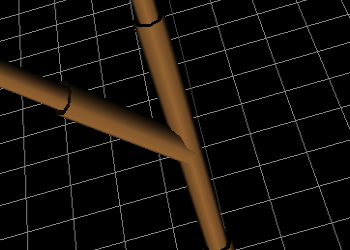
\includegraphics{fig/bijunct}
            \caption[Normal Bijunction]{The result of a normal bijunction production}
            \label{fig:fig/bijunct}

        \end{figure}
        \item Forked bijunction: Branch splits into two, with both diverging at a small acute angle
from the previous vector. See figure \ref{fig:fig/fbijunct}.
        \begin{figure}[h]
            \centering
            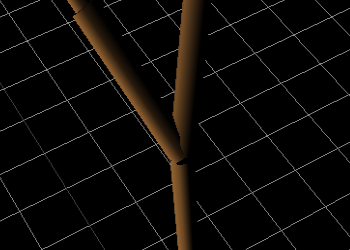
\includegraphics{fig/fbijunct}
            \caption[Forked Bijunction]{The result of a forked bijunction production}
            \label{fig:fig/fbijunct}

        \end{figure}
        \item Pseudo-trijunction: One branch from a trijunction is moved down the parent
branch, resulting in a normal bijunction stacked below a fork bijunction. See figure
\ref{fig:fig/pseudotri}.
        \begin{figure}[h]
            \centering
            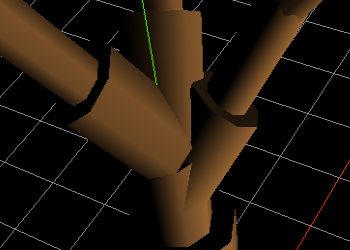
\includegraphics{fig/pseudotri}
            \caption[Pseudo-Trijunction]{The result of a pseudo-trijunction production}
            \label{fig:fig/pseudotri}

        \end{figure}
    \end{itemize}

            \subsubsection{Density Management}
    \tab To manage the spacing of trees in the generated forest, forest system models will be
adapted, with additional logic to make them appropriate for a visual output. As discussed above,
forest gap models break forests up into tree grids, corresponding roughly to the area of affect of
the canopy trees\cite{moorcroft01}. The grids operate under a set of assumptions\cite{bugmann01},
some which must be reconsidered for a visual output:
\begin{enumerate}
    \item The forest is abstracted as a composite of many small patches of land, where each can
have a different age and successional stage.
    \item Patches are horizontally homogeneous, meaning the tree position within a patch is not
considered.
    \item The leaves of each tree are located in an indefinitely thin layer at the top of the stem.
    \item There are no interaction between patches.
\end{enumerate}
    \tab Obviously, assumption \#2 must be violated for a visual output: horizontal position in the
patch is exactly what we do care about when attempting to manage the density of the forest. As,
by the model, the position of trees in the patch doesn't matter, however, we can conclude that the position of the canopy
trees in the patch doesn't matter, and can be assigned randomly. Furthermore, I will make the
assumption that only a single tree in each patch is canopy-tree-sized. Assumption \#4 suggests a
few problems in the system, which will be addressed at the end of the section.

    \tab Thus, we begin the algorithm by following assumption \#1, dividing the terrain area up
into patches. The size of these patches is the subject of disagreement, ranging from the order of
$10m^{2}$\cite{moorcroft01} to $1km^{2}$\cite{bugmann01}. I will assume that the former is true:
the size of a patch is dictated by the canopy size of the canopy trees. This size is dictated by
size and height of a tree, which is roughly correlated with the age of the tree. The L-System used
to generate the trees in this project uses recursion depth as a rough stand-in for tree age; thus,
the value assigned as the max recursion depth will be used to dictate the size of a patch. We can
use this value, along with maximal values for branch length and branching angle, to set an upper
bound on the size of the canopy. The equation governing the maximum canopy size is:
% Get figure using eps or pdf, use vectored graphics
% Write about grid artefact


\begin{displaymath}
    \text{max\_canopy} = 2  D  L \sin(\alpha)
\end{displaymath}
Where $D$ is the maximum recursion depth of the L-System, $L$ is the maximum length of a branch,
and $\alpha$ is the maximum branching angle. I will assume that the root system of the tree
behaves similarly to the branch system, allowing the canopy to singly govern the size of the patch.
Thus, the algorithm will begin by dividing the terrain into patches of size \verb|max_canopy|.
Following my discussion of assumption \#2, a tree which will be rendered to maximum depth,
making it a canopy tree, will be placed randomly in each patch. From here, smaller trees could be
seeded; this will be discussed in the section on extensions. This implementation allows the details
of forest generation, specifically any constants relating to how the forest is created, to be
dictated entirely by the trees used in the forest, which prevents the user from having to supply
additional detail about forest construction and allows for a very clean implementation of the
\verb|Forest| module.

    \tab A major problem with this algorithm is suggested by assumption \#4: there is nothing
preventing two trees from existing close to their shared border, thus growing unrealistically close
together, or even colliding. A possible solution to this bug will be discussed in the
aforementioned section on extensions; for now, however, I leave this visual error up to chance.

        \subsection{Tree Implementation}
    \tab The creation of a tree begins by constructing a rule set for the L-System. A few of these are
defined in \verb|./js/app/lsys_rules.js|, which can be used as an example for users wishing to
create their own L-Systems. This rule set is used to create an L-System object, which will be used
to generate the tree's geometry. A turtle must also be constructed and tied to the Three.js library
in order to draw to the HTML5 canvas. Then, by calling the L-System object's
\verb|build()| method, the L-System will recursively construct a tree, storing it in its own
\verb|system| variable. The built L-System is then passed into the turtle object's \verb|run()| method,
which will draw the constructed L-System as a single hierarchical object onto the HTML5 canvas.

            \subsubsection{turtle\_graphics.js}
    \tab The turtle graphics module consists of a turtle object, \verb|Turtle|, a set of turtle
commands to control drawing, and a \verb|run| method, which, given a list of turtle commands,
executes them in order from the current position.
\begin{itemize}
    \item \verb|Turtle(scene, material, radius)|: Turtle object constructor. Creates the turtle
drawer, initializing it at the world origin oriented in the $+y$ direction. Turtle properties
are as follows:
    \begin{enumerate}
        \item \verb|rate|: Defaults to 1. Rate at which turtle travels when moving forward,
    multiplied by the forward command's \verb|time| parameter to get the total distance traveled.
        \item \verb|width|: ``Width" of the drawn line. Defaults to 0.25, can be passed in as an
    argument. Actual value is the radius of the cylinder primitive created by the turtle.
        \item \verb|scene|: Three.js scene. Required. Graphics drawn in \verb|run()| are
    added to this as a single, hierarchical object.
        \item \verb|material|: Three.js material. Required. Defines the material of the
    drawn cylinder lines.
    \end{enumerate}

    \item Turtle commands: The turtle commands (\verb|_F()|, \verb|_f()|, \verb|_pitch()|,
\verb|_yaw()|, \verb|_roll()|, \verb|_push()|, \verb|_pop()|, and \verb|_set()|) are all methods
that specify commands to some turtle object. To use, they are attached to a \verb|Turtle.Action|
object along with the value of their argument, and then passed as a list as the argument to
\verb|run()|. Each one specifies a action relative to the turtle drawer's current position and
orientation. Details of the actions are given in table 1. The rotation actions work by
multiplying a specific rotation matrix to the turtle object's internal orientation matrix. The use
of a rotation matrix allows for relative transforms, as opposed to Euler coordinates, which require
a specific ordering of rotations that can lead to errors. The forward movement controls drawing; it
does this by creating a cylinder of the current width and given distance (the actual given is a
time parameter, which is multiplied by the turtle's \verb|rate| to get the cylinder's length) and
moving it such that it begins at the turtle's starting position and is oriented in the same
direction of the turtle. Then, the turtle's position is incremented by the given distance.
\verb|_push()| and \verb|_pop()| save the turtle's state in a basic object and store or retrieve it
from an internal stack.

    \item \verb|run()|: The run commands executes a given turtle string. Looping through the string
in order, it run's the function's built-in \verb|call()| function, specifying \verb|this| as the
calling object and \verb|Turtle.Action.args| as the arguments. This binds the current turtle object
to the action, allowing the turtle command to affect the turtle object's internal variables.

\end{itemize}
            \subsubsection{lsys.js}
    \tab \verb|lsys.js| is used to describe and create an L-System of arbitrary
productions and rule set. Relevant objects, including \verb|LSystem.Production| and
\verb|LSystem.RuleSet|, are defined, and the engine to run recursion to a specific depth is
included in a method of the base \verb|LSystem| object. The L-System requires both a rule set and
an initial value to run, both of which are described below.

\begin{itemize}
    \item \verb|LSystem|: Object containing the L-System and its rule set. The only argument is
\verb|rule_table|, the rule set for the L-System.
    \item \verb|LSystem.Production|: Object containing production information. Productions, with
the added information of their rule sets, represent a specific type of growth, but are not actually
drawn by the turtle graphics wrapper. Production arguments are as follows:
    \begin{enumerate}
        \item \verb|id|: ID of the production, similar to function name. For example, in the
production A(1,4), the id is ``A".
        \item \verb|args|: List of argument values. This is only assigned for initial values; the
\verb|inject| function is used to dynamically assign these values, as the resultant value is
usually some function of the previous value, defined in the rule set.
        \item \verb|inject_args|: Function used to dynamically assign arguments from within the
rule set. Arguments after the replacement step are usually a function of their previous values;
the width of branches, for example, might decrease by a constant scale at each level of branching.
The function must take \verb|args|, the previous production's arguments, and \verb|consts|, a
dictionary of constants defined in the rule set. It must then assign \verb|this.args| to a list of
the argument values. This method can also be used to implement parameter variation, which is also
calculated dynamically, with a random value and specified range.

    \end{enumerate}
    \item \verb|LSystem.RuleSet| and \verb|LSystem.Rule|: \verb|RuleSet| and \verb|Rule| are used
to define the logic of the L-System. \verb|RuleSet| describes the entire rule system, whereas \verb|Rule|
defines a single rule for a specific production and condition. The arguments for the \verb|RuleSet|
constructor are as follows:
    \begin{enumerate}
        \item \verb|consts|: Dictionary of defined constants, such as width reduction ratios, used
    in calculating the argument values at replacement.
        \item \verb|initial|: Initial production list values for the system.
        \item \verb|rules|: List of rule objects for this system.
See \verb|lsys_rule.js| and its below explanation for more details on \verb|LSystem.RuleSet|
construction.

    \end{enumerate}
The arguments for the \verb|Rule| constructor are as follows:
    \begin{enumerate}
        \item \verb|id|: ID corresponding to the production this rule affects.
        \item \verb|condition|: Condition function to the parametric term. Function takes as
    argument the production object and returns a boolean. Allows the rule to match on the
    value of the production's parameter. 
        \item \verb|output|: List of production and turtle action objects to replace the matched
    production with upon recursion. 

    \end{enumerate}
More details about the construction of a \verb|RuleSet| can be seen in the documentation for
\verb|lsys_rule.js|.

    \item \verb|build()|: Launcher function for the recursive L-System construction. Calls internal
recursion function on each element in the initial system; thus, it requires that the \verb|system|
variable is set to a list of initial values. The internal recursion runs for a single object in the
system list, matching it to the rule set and replacing it with the appropriate output string. It
then recursively calls itself on each element of the output array, to a specified \verb|MAX_DEPTH|
value. Optional argument \verb|debug| is a boolean that toggles printing of the constructed system
after construction.

    \item \verb|checkRule()|: Function that checks a given element of the system against the
system's rule set, returning the appropriate output. Does a linear search through the list of
rules, halting when a match occurs. Matches require that both the rule id and the production id
match, as well as the rule's \verb|condition| function returning a \verb|true|. The rule's output
is then cloned to avoid problems with Javascript's singleton objects affecting subsequent
production values. The arguments are then injected using the production's provided
\verb|inject_args| function, which allows dynamic evaluation of the arguments based on the
previous production. The output is then returned. If no match is found, the initial production is
returned unchanged.

    \item \verb|printSystem()|: Used for debugging. Pretty prints the current value of the
L-System's \verb|system| variable, in form \verb|id(args...)|. Activated when the \verb|debug| flag is
turned on in \verb|build()|.

\end{itemize}

            \subsubsection{lsys\_rule.js}
    \tab \verb|lsys_rule.js| provides a convenient package of L-System rules used in \emph{The
Algorithmic Beauty of Plants}\cite{abp96}. The rules found in it are used to create the trees in the final
Garden of Eden project, but can also serve as examples to users wishing to generate their own
L-Systems. The structure for a rule set is given in the above description of
\verb|LSystem.RuleSet|.
    \begin{itemize}
        \item \verb|HondaTree|: Creates an object that inherits from \verb|LSystem.RuleSet|.
Description of a Honda L-System comes from H. Honda\cite{honda71}. The tree is of a constant
height, but branches with increasing detail at higher levels of recursion. Defined constants allow
for a decent amount of variation on what is otherwise a visually highly symmetrical tree.

        \item \verb|TernaryTree|: Creates an object that inherits from \verb|LSystem.RuleSet|.
Description of a Ternary L-System comes from P. Prusinkiewicz et al.\cite{abp96}. By using L-System
rules that match to turtle commands, this tree actually grows both larger and more detailed at
higher levels of recursion, which more closely resembles the growth of a tree. There is only one
branching rule, which uses a trijunction at each branching node. The generated tree is
visually quite complex, but has some symmetrical artefacts visible from specific angles. Varying
constants allows for a large amount of variation on this tree structure.

        \item \verb|RandomTree|: Creates an object that is an extension of the rule set defined in
\verb|TernaryTree|, but with the randomization features discussed in this thesis. This is the tree
rule set used in the Garden of Eden.

    \end{itemize}

    \subsection{Forest Implementation}
    \tab The \verb|Forest| module manages the placement of trees, as well as running their
generation and rendering. As such, it is the top-level module for Garden of Eden. It does this in
two cycles, \verb|plant()| and \verb|grow()|, which are discussed below. Several significant
extensions to this module are mentioned in the section on extensions.
\begin{itemize}
    \item \verb|Forest(geography, scene)|: Constructor for the \verb|Forest| module.
\verb|geography| argument is a generated \verb|Terrain|. \verb|scene| is a Three.js scene, to which
the trees will be added.

    \item \verb|addSpecies()|: Method to add L-Systems, representing different tree species, to the
forest. Currently, only the first L-System in the list is used; an extension to this is discussed.

    \item \verb|build()|: Top-level method for the \verb|Forest|. Calls \verb|plant()|, then
\verb|grow()|. Many of the extensions, especially growth time emulation, would involve significant
changes to this method, as it currently only has the most basic possible functionality.

    \item \verb|plant()|: Runs the density management algorithm. Using the L-System provided by
\verb|addSpecies()|, calculates the patch size for this forest. Then, looping through all patches,
creates a single \verb|Turtle| at a random location within the patch as well as an L-System seeded
with the given rule set, saving both to a list of trees. Run time is very fast, as it simply sets up
the more time-intensive calculation for \verb|grow()|.

    \item \verb|grow()|: Runs all of the generation and rendering tasks for each tree, thus being
the predominant limiter of run time. First, it empties the species list to free that memory. Then,
popping each tree from the list of trees, again to free up memory on completion, \verb|grow()|
first builds the tree's provided L-System, then runs the turtle commands to create the Three.js
tree. It then drops the tree onto the terrain below, sending a notice to the console upon
completion. While simple, as mentioned, this method is a massive draw on computational resources,
and thus would greatly benefit from run time improvement.

\end{itemize}

    \section{Outstanding Issues}
        \subsection{Memory and Run Time}
    \tab Currently, memory use and run time are a major issue when generating and rendering large
forest scenes. The memory issue stems from both a liberal use of objects throughout the code, as
well as the unavoidable exponential nature of tree geometry. Run time seems to be largely
tied to the growth phase of the forest cycle, suggesting either a re-write of the turtle graphics
module or limitations of Three.js.

            % Different object representations, matrix, cylinder transform
            % Cylinder transformations
            \subsubsection{Data Structures}
    \tab One of the significant memory problems is the use of object-dense data structures
in intermediate and final representations of tree structures. Objects, while logically useful for
code design, are not optimized for memory use; thus, the large number of objects used in Garden of
Eden, representing everything from a single turtle action to a single twig, suck up memory
resources and tie up computation time in garbage collection. Thus, a re-design of data structures
would greatly benefit both memory use and run time.

    \tab The proposed redesign is a departure from the use of turtle graphics to represent
the transition from growth to visual rendering. The turtle graphics representation of Three.js
primitives is both incredibly object dense and unnecessarily verbose, leading to very poor use of
memory. Turtle graphics are a simple way to describe a drawing action, but for the specific case
of trees, this drawing representation is unnecessary, as a direct representation of the branches could be
used instead. Trees are simply a collection of cylinders of
different size, shape, position, and orientation; thus, a more condensed representation could be
constructed of a set of cylinder transforms. The same L-System replacement action could apply, but
instead of a set of drawing commands, a simple list of numbers could be replaced, representing
new cylinder primitives. This could take the form of a heap, with a fixed number of values
representing each branch: $(\text{index}, r, \phi, \theta, w)$. Index is a value that represents
the root branch of the given segment, with index 0 being the initial position. This would allow for
position values to be dropped from the list, as everything is defined relatively to previous
branches, with only an initial position of the tree required to place the whole thing in space.
Thus, an entire forest of trees could be represented in a very compact array, minimizing memory use
and still allowing for $\Theta(n)$ run-time for primitive construction.

            \subsubsection{Geometry}
    \tab Another, simple data structure redesign is built in to Three.js. The primitive type
currently used, \verb|CylinderGeometry|, is an extension of Three.js's core \verb|Geometry| object,
an object-based prototype that allows for the construction of arbitrary shapes via vertices and
faces. There is, however, a more optimized option: \verb|BufferGeometry|, a buffered representation
of the same geometry that saves on memory and CPU cycles. It is more difficult to work with, but
there exist methods to convert regular \verb|Geometry| objects to the more efficient
\verb|BufferedGeometry| objects. It could also be manipulated directly, constructing a tree by adding
vertices and faces instead of cylinders, for a much more condensed tree primitive.

            \subsubsection{Parallelism}
    \tab An avenue for increased computational efficiency that was unable to be explored, due to
limitations in Javascript, was parallel processing of the tree generation process. By setting up a
generator and workers, the branches of the tree could be solved independently, on multiple cores or
multiple workstations, resulting in a large decrease in the total computation time. As Javascript
does not support parallelism, this parallel characteristic of tree geometry was unable to be
utilized; however, if the tree API discussed in the extensions implemented the tree creation in a
different language, massive improvements could be seen with appropriate application of parallel
methods.

        \subsection{Density Management}
    \tab Currently, the density management module has a potential error in tree collisions. This
will be discussed in detail in the extensions section.

    \section{Extensions}
        \subsection{Tree Rendering}
    \tab Currently, there is a significant user experience issue in the time it takes to properly
render out a forest of trees. The current solution ignores this, expecting the user to patiently
wait several minutes for the trees to render into a forest. Extensions to address this issue,
either by speeding up the processs or by circumventing the issue, are proposed below.

            \subsubsection{Pre-Rendering}
    \tab Pre-Rendering involves setting the project up with a basic framework to allow for database
storage of tree primatives. This solution would save generated tree structures, populating a forest
directly from the database upon reaching the page instead of running the full generation cycle.

    \tab Several problems arise with this solution. First, prototype data is lost when serializing a
Javascript object to JSON. Thus, a special serialization process would need to be created in order
to store the Three.js graphical primitives. Furthermore, as the objects would be created out of
environmental context, growth affectors such as global and local tropism would not be able to
affect the geometry of the trees produced.

    \tab The benefits of the solution, however, are significant. The user wait time would likely be
negligible, allowing the experience to being almost immediately upon accessing the site. For
today's impatient users, this is extremely important. Additionally, the addition of a database\
could open up extensions such as saving particularly nice generated forests.

            \subsubsection{Background Rendering}
    \tab Javascript does not support threading; however, several worker queue libraries exist that
could allow for the creation of trees to happen asynchronously to the creation of the Three.js
scene. The user would open the page to a freshly generated, but empty, terrain; as they explore,
fully-grown trees would appear around them as the workers finish. The materialization effect would be
somewhat jarring, but this could be artistically mitigated with clever visual distraction, such as
thick fog with increasing visibility as trees appear. See also the below section on Growth Time
Emulation, which could be used in conjunction with this acceleration process.

            \subsubsection{Tree API}
    \tab While Javascript does not allow local threading, it has significant asynchronization
support in AJAX. To take advantage of this, a tree API could be written. This would have an effect
similar to Background Rendering, except that it would utilize default Javascript functionality
instead of a third party library. 
Furthermore, there is nothing forcing the API server to use a language that doesn't support
threading; the generation could be written in a much faster language, utilizing parallelism and 
outputting carefully
serialized Three.js objects as an asynchronous HTTP JSON response. Global forest data could also be
supported by being included as a parameter to the AJAX request to the API.

        \subsection{Graphical Primitives}
    \tab The current primitive used by the turtle graphics wrapper is a basic cylinder, of diameter
specified by \verb|Turtle._set()| and length specified by \verb|Turtle._F()| and the turtle's
speed. This results in a very noticeably blocky tree, where each branch has a discontinuous shift
in diameter. Obviously, trees in nature to not display such structure; thus, using a different
graphical primitive would result in a much more realistic-looking tree.

            \subsubsection{Tapered Cylinder}
    \tab To create a tapered cylinder, the turtle's forward draw command would need to take in to
account two \verb|Turtle._set()| commands, using them in conjunction with Three.js's cylinder
pyramid to make a conical frustum. By matching the diameter of the top of one branch with the
diameter of the bottom of the next, the branches of the tree would blend together, resulting in the
continuous look found in nature.

    \tab To do this, a new turtle command would need to be implemented. \verb|Turtle._Ft()| would
work similarly to \verb|Turtle._F()|, except that it would use a conic frustum as a primitive. The below row
expands on Table \ref{tab:turtle}.
\begin{table}[h]
\centering
\begin{tabular}{|l|l|l|p{7cm}|}
    \hline
    Command & Symbol & Argument & Description \\ \hline \hline
    \_Ft & Ft & time, width & Moves turtle forward by specified time value. Draws line as a conic
frustum beginning with the turtle's current diameter and ending at the specified diameter. Also
sets the turtle's diameter to the specified diameter.\\ \hline
\end{tabular}
\caption[Taper Command]{Turtle Taper Command}
\label{tab:taper}
\end{table}

            \subsubsection{Extruded Line}
    \tab Another option for smoothing the discontinuities is using Three.js is to use the extruded
shape feature of Three.js, using a \verb|THREE.CurvePath| to represent a path. There are several
benefits to this option. Extruded paths support tapering lines by default, which would allow a
branch to be represented as a simple, light-weight path. A collection of paths might be able to be
extruded in a single step, which could improve rendering time. Visually, this would be a very good
option, as the extrusion process would smooth the branch joints, which currently are merely the
intersection of cylinder primitives and are discontinuous. Using an extruded line might also allow
for branch bending; as discussed in Section \ref{subsubsec:assumptions}, branches are currently
assumed to be perfectly straight, whereas real branches are usually curved to some degree.
Representing branches as paths would allow for the manipulation of these paths, resulting in a
extruded branch with a visually more accurately curved shape.

    \tab The process of creating these paths, however, might be difficult. It might be
useful, as with the tapered cylinder, to implement another turtle command that takes as an argument
a tapering constant. Post-processing of the turtle command list might also generate data to feed to
the extruded shape constructor, adding a large list traversal but allowing the user to implement it
without using an L-System constructed with extrusion rules. The details of this implementation,
however, will be left for future consideration.

        \subsection{Tropism}
    \tab Defined biologically as growth in response to a biological stimulus, an implementation of
a tree's response to lighting conditions, called \emph{heliotropism}, and the proximity of other
trees could result in a more realistic representation of a forest ecosystem. A simple way to
represent tropism is by calculating an orientation adjustment, $\alpha$, the formula for which is
given below:\cite{abp96}
    \begin{displaymath}
        \alpha = e | \overrightarrow{H} \times \overrightarrow{T} |
    \end{displaymath}
Where $H$ is a vector representing the branch, $T$ is a vector representing the tropism on the
tree, $|T|$ is the strength of influence of the tropism, and $e$ is a constant representing the
susceptibility of a branch to the effects of tropism.

    \tab Thus, a vector must be found to represent tropism on the tree. This could easily be
handled by the forest model: a global vector could represent the prevailing light conditions of the
area, which would then be averaged with a per-tree vector representing the local effects of tree
proximity to get the vector $T$.

        \subsection{Path Traveling}
    \tab A significant design consideration when making this project is the unique interactive
experience, especially with regards to modern video games. If this project is to be considered a
game, then the ``objective" is not anything tangible, creative, or destructive; instead, I wish to
effect a whimsical sense of exploration, reminiscent of childlike play in nature. The user is not
in control of their environment; in many ways, I hope that this lack of agency inspires a sense of
curious awe.

    \tab To this end, I would consider removing, or at least limiting, the user's ability to
navigate the world. The current hosted version significantly limits user navigation speed and
disables jumping, attempting to ``slow down" the experience and force the user to focus on the
scene instead of navigation concerns and the thrill of speed. An interesting extension, however,
would be using path-finding algorithms to control, or at least guide, user navigation. 

    \tab One possible implementation would be to bias the user movement with a pathfinding
algorithm, allowing user control only as slight deviations from the path. Thus user would thus be
allowed a small amount of control over their exploration, but would ultimately be pulled towards
the calculated path. Alternatively, movement controls could be disabled completely, allowing the
user only to look around as they are led on a walk around the forest.

    \tab Several pathfinding algorithms exist for consideration. Dijkstra's algorithm, for example,
or its extension A*, are designed to find the shortest path in a graph, and can be used to
calculate a path around obstacles. However, these algorithms are designed to find a shortest path;
in this case, as the journey is more important than the destination, I propose an alternative
algorithm, based on Namco's Pac-Man\cite{pittman11}. As the user travels, a random ``target point"
shall be calculated. Then, the player is moved steadily towards that point, using weighted-vector
calculations. This weighted vector would tend to point directly toward the target point, but would
be deflected by nearby trees. The action can be thought of as similar to a charged particle moving
towards a strong attractor, but repulsed by nearby point charges. The user would thus move to
the most open areas that lead towards the target point; this has an appealing element of realism to
it, as people tend to travel through forest following perceived ``paths", which are usually
locations of most negative space between trees. When the user arrives at or near the target point,
a new target point will be calculated, forcing the user into perpetual motion.

        \subsection{Feature Extraction}
    \tab The feature extraction method, from N. Yokoya et al.\cite{yokoya89}, is a fairly involved
process that requires finding actual topography data from a representative terrain and building an
analytical program that runs statistics on the output of a fractal function with reference to the
slope grades found in the representative surface. It would result in a set of justifiably accurate
constants, which would render a random fractal surface that was similar to the representative real
surface. These constants include the fractal ``roughness" factor, as well as a range of scales for
which the fractal representation of topography is realistic. As it was deemed a significant tangent
from the focus of the thesis, however, this method was not pursued.

        \subsection{Erosion Emulation}
    \tab Erosion emulation\cite{mustgrave89} is a process by which generated terrain can gain the a little
appearance of natural weathering. Currently, terrain is passed through a Gaussian filter, a
low-pass filter that smooths over small-scale bumps while preserving larger features. This is
visually effective at removing terrain noise, which is annoying to the user whose height changes
with respect to the terrain, causing a ``bumpy" oscillation of the camera; however, it is not
naturally justified. Erosion emulation would be more effective: a natural low-pass filter, it would
smooth over annoying terrain noise while giving the scene a cool sense of natural age.

        \subsection{Tree Species}
    \tab Currently, only a single, archetypal tree is being created by the specified L-System.
Obviously, the forests usually consist of different species of trees growing together. This could
easily be implemented by including a set of L-System rules, each representing a different tree
species. The species could be randomly selected upon the \verb|Forest|'s seeding step, or, if a
dominant species is desired, such as is found in a pine forest, probability could be assigned to
each species. A more sophisticated selection algorithm could take in to consideration biological
advantage for resource aquisition; for example, a tree predisposed to grow taller might be better
at capturing light. Careful consideration when constructing the L-System ruleset should be taken if
specific species are desired, but a significant body of literature exists discussing the
topological details of different tree species.

        \subsection{Texturing}
    \tab Current, Garden of Eden almost entirely uses solid colors for a very simple look. The use
of some basic textures would make the rendered scene look nicer and more realistic.

            \subsubsection{Bark}
    \tab A basic, brown bark texture would be a significant visual improvement over the current
solid mesh. This texture could come from images of real trees, which might result in very realistic
bark; however, the texture should be wrappable in order to avoid seam artefacts. Thus, a bark
generation method\cite{bloomenthal85} might be preferable. The proposed method uses sawtooth waves
and coloration to achieve a decently-realistic bark look that is wrappable in all directions.

            \subsubsection{Bump Map}
    \tab Currently, branches are represented as straight, smooth cylinders. Branches in nature,
however, are twisted, gnarled, and scarred. This effect can be achieved with a bump map texture,
which could be generated with the bark texture to produce the appropriate visual. This could also
be used to simulate burls and broken branches, which could be generated along with the actual
branches in the L-System, to be rendered out by the texture engine. 

        \subsection{Growth Time Emulation}
    \tab The L-System used for the trees in Garden of Eden has replacement rules for both
productions and turtle commands; in other words, it affects both branching junctions and the length
and width of the rendered branches. Thus, the branches grow with time, offering a rough correlation
between depth of recursion and age of the tree. This extension seeks to expand on this correlation,
growing the trees in a process that actually represents time, or the age of the tree in question.
A single level of recursion, for example, might represent a year of growth. This would open up a
lot of different avenues of forest growth representation. Growth events, mentioned below, become
possible. The working assumption that all trees are of a roughly evuivalent age could also be
broken: the seeding and growth step could occur in parallel, resulting in a forest of trees and
their sapling progeny.

    \tab This extension would require a significant rewrite of the \verb|Forest| module and a
specially written L-System ruleset. The \verb|Forest| module, with the backgrounded workflow
described above, would need to combine the seeding and growing steps. This could involve a
significant amount of IPC, which Javascript does not easily support. It therefore might work better
in conjunction with the Tree API setup, which could provide solid backgrounding support as well as
the IPC required for growth time emulation.

        \subsection{Density Management}
    \tab There are a few problems with the current density management implementation, which will be
addressed in detail below. There exists a non-deterministic (due to the use of random placement)
bug where trees placed might be too close, or even in contact with, trees in adjacent patches.
Furthermore, the algorithm used easily and logically supports the addition of younger trees to fill
out the patch.

            \subsubsection{Seedlings}
    \tab The current density management system lends itself well to extension with regards to
adding new, younger trees to a given patch. The process should take in to consideration the
distance from the canopy tree, as the dominant tree in the patch should get most of the resources,
and preventing young trees from growing too close to the canopy tree would prevent tree collisions
from occurring. I propose modeling the patch as a particle system, with the canopy tree as a source
of repulsion, and deriving a probability of elimination from the inverse square law thus derived.
A constant amount of seedlings would be placed randomly in the patch, perhaps as a part of a growth
time emulation step. Then, using the above inverse square law, the seedlings would be filtered on
their derived probability. This would make the density manager follow the gap models on which it is
based much more accurately, in addition to improving the realism of the generated forest by
breaking the same-age assumption.

            \subsubsection{Placement Error}
    \tab The aforementioned placement error arises from breaking the assumption that patches are
horizontally homogeneous, and that there are no interactions between patches. This can lead to an
error where trees are placed close to a shared border, resulting in collision of the trees that is
either unreasonable or impossible. There are two possible solutions to this problem:
\begin{enumerate}
    \item Edge repulsion: Similar to the seedlings problem, an inverse square law would be used to
repulse canopy trees away from the edges of the patch, resulting in a placement distribution
strongly biased towards the center of the square. This would combine well with the proposed
seedling extension and offer a probabilistic solution, which has been used throughout the problem
as a stand-in for natural, deterministic methods.

    \item Closest pair algorithm: A more direct solution would be to use a closest pair
algorithm\cite{kramii14} to obtain a list of trees that violate visual or natural closeness
constraints, then filtering said list to remove collisions. The below algorithm is a linear
solution to the problem:
\begin{alltt}
Gaussian-Density-Management(density)
    // Proximity detection step
    Create a grid where each square is half the distance between trees, calculated
        from the density
    Seed grid with first tree by mapping the tree's location to the grid and adding
        it to that spot
    For every subsequent tree \(t_{dest}\),
        Map tree location to grid
        If there are any trees mapped to that location or any of its compass neighbors,
            For each neighboring tree \(t_{src}\),
                Calculate the Euclidean distance between \(t_{src}\) and \(t_{dest}\)
                Construct a pair of \(t_{src}\) and \(t_{dest}\), including the calculated
                    distance
                Add pair to a list of pairs

    // Filter step
    For each pair in the pair list
        map distance to normal curve to get probability
        filter using that probability
    \end{alltt}
    \tab The algorithm fits well with the current density management system in that it partitions
the terrain plane into a grid, though of a different size than the patches used to place canopy
trees. However, it is a somewhat hacky solution, as it only fixes the bug as it occurs, instead of
finding a more natural solution to prevent it.

% Subgrids

\end{enumerate}


        \subsection{Growth Events}
    \tab Growth events are defined generally as any effectively instantaneous event that
dramatically affects tree growth. Growth events could include, but are not limited to, weather
affects such as wind damage or lightning, disease, or damage from other trees. These effects are a
random, singular event that can significantly change the visual appearance and factors affecting
the growth of a tree, and that don't necessarily have global affects. These events could be
randomly simulated in the aforementioned growth time emulation, with a random event affecting a
single, random tree at a specific interval. The result might range from truncated branches to split
trunks, even complete removal of the tree. They would, however, have to occur during the L-System
recursion, and would require significant rewriting of the recursion structures to handle outside
affectors. 

    % ADD what I learned?

    %\nocite{*}
    \bibliographystyle{plain} % abbrev?
    % dblpp
    \bibliography{refs}
\end{document}


% Questions:
% Should I label all sections referred to, or can I use terms like "aforementioned"?
